% ====================================================
%   Copyright (C)2019 All rights reserved.
%
%   Author        : Xin-Xin Ma
%   Email         : xxmawhu@163.com
%   File Name     : spinPrece.tex
%   Last Modified : 2020-01-16 16:37
%   Describe      :
%
% ====================================================%
\chapter{研究超子在磁场中的进动效应}
\section{简介}%
本章节我们将研究超子对的产生特点。以$e^{+}e^{-} \to J/\psi \to \Lambda \bar{\Lambda}$为例做研究,
这是因为这个过程受到了广泛关注,并且过程简单又能够有效的说明问题。
考虑到$\Lambda$ ($\bar{\Lambda}$)具有一定的磁矩,因此其自旋方向受磁场的影响。北京谱仪内部恰好有
一个强度为1T的磁场,故推断$\Lambda$ ($\bar{\Lambda}$)的自旋方向将会绕着磁场做转动,这意味
着$\Lambda$ ($\bar{\Lambda}$)衰变时刻的自旋方向将不同于产生时刻的,这将导致整体末态角分布发生变化。
然而实验上\cite{Ablikim:2018zay, Ireland:2019uja, Ablikim:2017tys,
Ablikim:2005cda,Aubert:2007uf, Ablikim:2012bw, Aubert:2009am}都忽略了这一点差异,这会对实验结果造成潜在的测量偏差。在下面的小节里,
我们首先给出讨论实验上所用的角分布,并给出修正项,接着进行实验模拟以定量的研究忽略修正项带来测量偏差。

\section{实验研究现状}
在北京谱仪采集到的十三亿$J/\psi$的样本的基础上,合作组对
$\Lambda$的衰变参数$\alpha_{-}$进行了最精确的测量,实验结果为 $0.750 \pm 0.009 \pm 0.004$~\cite{Ablikim:2018zay},
出乎意料的和世界平均测量值偏离了7$\sigma$,这修正了一系列的实验测量结果。
在2019年,文献\cite{Ireland:2019uja}利用CLAS的数据重新测量了$\alpha_{-}$,结果和BESIII的偏离为2$\sigma$。
目前这两个实验都没有考虑到$\Lambda$在磁场中的进动,这也是本章研究的一个出发点。以北京谱仪为例,
考虑到束流能量和$\Lambda$的寿命,很容易得到$\Lambda$在探测器内部的平均飞行距离为12cm,相应的进动角约
为1$^o$。进动的角度虽然小,但是实验的精度很高。在实验\cite{Holmstrom:2004ar}中对$\Xi^{-}$的$CP$破坏测量
精度已经达到了$10^{-4}$,在未来的超级粲-陶工厂中,对超子衰变$CP$破坏的灵敏度将达到$10^{-4}$
到$10^{-5}$\cite{Bigi:2017eni},在这种精度下,忽略磁场带来的进动将是致命的。

\section{$\Lambda\bar{\Lambda}$对的产生}
在北京谱仪上,相干的$\Lambda \bar{\Lambda}$通过级联过程$e^+e^- \to J/\psi \to \Lambda \bar{\Lambda}$产生。
有效振幅为
\begin{equation}
    \begin{split}
        M &= \frac{ie^2}{q^{2}} j_{\mu} \bar{u}(p_{1}, s_1) \left( F^H_1(q^2) \gamma_{\mu} +
        \frac{F^H_2(q^2)}{2m_{\Lambda}} p_{\nu} \sigma^{\nu\mu}  \gamma_5 \right) \\
        & \times \nu(p_2, s_2),
    \end{split}
\end{equation}
式中的$p_1$ ($p_2$)表示$\Lambda$ ($\bar{\Lambda}$)的动量, 
$m_{\Lambda}$是$\Lambda$的质量,$s_1$ ($s_2$)为$\Lambda$ ($\bar{\Lambda}$)的自旋矢量, 
转移动量$q = p_{1} + p_{2}$, $p = p_{1} - p_{2}$, $s = p^{2}$,
$j_{\mu} = \bar{u}(k_1) \gamma_{\mu} \nu(k_2)$是轻子流其中的$k_{1}$ ($k_{2}$)
是$e^{-}$ ($e^{+}$)的动量。 
需要特别指出的是形状因子$G^H_{E}$和$G^H_{M}$即所谓的强形状因子\cite{Faldt:2016qee},
这是由于$\Lambda\bar{\Lambda}$是通过$J/\psi$的强衰变产生的\cite{Faldt:2017kgy},与之相关的常用的
形式$F^H_{1,2}$的定义为
\begin{equation}
    G^H_{M} = F^H_1 + F^H_2,~G^H_{E} = F^H_1 + \tau F^H_2,
\end{equation}
其中$\tau = \frac{q^2}{4 m_{\Lambda}^2}$。
仿照文献\cite{Dubnickova:1992ii,Gakh:2005hh,Czyz:2007wi}的方法,很容易得到微分截面为(丢掉了和角分布无关的常数):
\begin{equation}
\label{eq:jpsi_LL}
    \begin{split}
        \frac{d\sigma}{d \cos\theta}  \sim & 1+ \alpha _{\psi } \cos^2\theta
        + \sin ^2\theta \hat{s}_{1}^x \hat{s}_{2}^x
        + \alpha_{\psi} \sin^2\theta \hat{s}_{1}^y \hat{s}_{2}^y \\
        &- \left( \alpha_{\psi} +\cos^2 \theta  \right)\hat{s}_{1}^z \hat{s}_{2}^z
        + \sqrt{1-\alpha_{\psi}^2} \cos\Phi  \sin\theta \\
        & \times    \cos\theta
        \left( \hat{s}_{1}^x \hat{s}_{2}^z  - \hat{s}_{1}^z \hat{s}_{2}^x\right)
        +\sqrt{1-\alpha _{\psi}^2}
        \sin\Phi  \sin\theta \\
        & \times \cos\theta  (\hat{s}_{1}^y - \hat{s}_{2}^y),
    \end{split}
\end{equation}
式中的$\theta$是$e^{+}$和$\Lambda$飞行方向之间的夹角,
$\alpha_{\psi} = \frac{\tau |G_{M}|^{2} -  |G_{E}|^{2}}{\tau |G_{M}|^{2} + |G_{E}|^{2}}$,
$\hat{s}^{i}_1$ ($\hat{s}^{i}_2$) 是$\Lambda$ ($\bar{\Lambda}$) 在其母粒子质心系下的
自旋的方向的第$i$个分量(选择$\Lambda$ ($\bar{\Lambda}$)动量方向作为Z轴,
$\vec{p}_1 \times \vec{k}_2$ ($\vec{p}_2 \times \vec{k}_2$)作为Y轴)。
$\Phi$是两个形状因子之间的相位差,定义为
\begin{equation}
    \frac{G^H_{E}}{G^H_{M}} = e^{i \Phi} \left|\frac{G^H_{E}}{G^H_{M}} \right |.
\end{equation}

\section{$\Lambda$自旋方向的改变}
与实验\cite{Ablikim:2018zay}有所不同的是,我们根据外部的磁场大小计算了衰变时刻的自旋取向。
考虑到自旋转动角度较小,利用$\Lambda$磁矩与磁场的相互作用\cite{Sakurai:2011zz},可以得到:
\begin{equation}
\label{eq:retate-s-sp}
    \hat{s}'_{1} = \hat{s}_{1} + \omega \tau_{\Lambda} \hat{B}  \times
    \hat{s}_{1},
\end{equation}
式中$\hat{s}'_{1}$代表$\Lambda$在其质心系下的衰变时刻$\tau_{\Lambda}$的自旋取向,并把
$\Lambda$产生的时刻作为时间起始点,$\hat{B}$是在$\Lambda$质心系下的探测器磁场的方向,
$\omega$是$\Lambda$的自旋绕磁场转动的频率,这个频率依赖于磁场强度$B$和$\Lambda$的磁矩大小$\mu_{\Lambda}$,
关系为
\begin{equation}
    \omega  = - \frac{2 \mu_{\Lambda} B}{\hbar},
\end{equation}
如果取$\mu_{\Lambda} = -0.613 \pm 0.04 \mu_{N}$~\cite{PDG},$B=1T$,$\Lambda$的平均寿命
$\tau_{\Lambda} = 2.632 \times 10^{-10}$ s及其典型动量大小为1 GeV/$c$,那么容易计算得到进动角度大约
为$\mathcal{A}_{\rm rota} = \omega \tau_{\Lambda} =0.017$ rad,类似的可以计算出其他的长寿命的超子,
比如$\Xi$, $\Omega$, $\Sigma^{\pm}$等在磁场中进动的角度。

一旦正确的认识到$\Lambda$衰变时刻的自旋取向为$\hat{s}'_{1}$,就能写出过程$\Lambda \to p \pi^-$的振幅:
\begin{equation}
    |M_{1}|^{2} \sim 1 + \alpha_{-} \hat{s}'_{1} \cdot n_{p},
\end{equation}
式中的$n_p$是质子在$\Lambda$质心系下的飞行方向,$\alpha_{-}$就是$\Lambda$的衰变参数,
类似的$\alpha_{+}$是$\bar{\Lambda}$的相应的衰变参数,与之相关的常见的一种$CP$不对称观测量
为$A_{CP} = \frac{\alpha_{-} + \alpha_{+}}{\alpha_{-}- \alpha_{+}}$。 最近的$A_{CP}$测量的实验结果为:
$A_{CP} = -0.006 \pm 0.012 \pm 0.007$\cite{Ablikim:2018zay},  而基于标准模型的理论
预言的量级为$10^{-5}$\cite{Donoghue:1986hh, Tandean:2002vy}。

为了得到整体的微分截面,我们需要给出$\hat{s}_{1}$, $\hat{s}'_{1}$的具体变换关系,
考虑到欧拉转动矩阵元,可以将方程\ref{eq:retate-s-sp}展开为
\begin{equation}
    \left(
    \begin{array} {c}
        \hat{s}'^x_{1} \\
        \hat{s}'^y_{1} \\
        \hat{s}'^z_{1} \\
    \end{array}\right)
    =
    \left(%
    \begin{array}{ccc}
        1                       & - \mathcal{A}_{\rm rota} \hat{B}'_{z}  & \mathcal{A}_{\rm rota} \hat{B}'_{y}  \\
        \mathcal{A}_{\rm rota}  \hat{B}'_{z}  & 1                       & -\mathcal{A}_{\rm rota}\hat{B}'_{x} \\
        -\mathcal{A}_{\rm rota} \hat{B}'_{y} & \mathcal{A}_{\rm rota}   \hat{B}'_{x} & 1                      \\
    \end{array}
    \right)
    \left(%
    \begin{array} {c}
        \hat{s}^x_{1} \\
        \hat{s}^y_{1} \\
        \hat{s}^z_{1} \\
    \end{array}\right),
\end{equation}
这里的$n_{\Lambda}$ 代表$\Lambda$在$J/\psi$的静止系下的运动方向,$\hat{B}'=\hat{B} + (\gamma-1) (\hat{B} \cdot n_{\Lambda}) n_{\Lambda}  $为将探测器内的磁场$B$通过洛伦兹变换在$\Lambda$静止系下的大小\cite{landau1952the}。
\section{修正后的微分散射截面}
当对$\Lambda$的自旋求和时,需要运用其正交性,即
\begin{equation}
    <\hat{s}^{i} \hat{s}^{j} > = \delta^{ij}
\end{equation}
这样很容易求得总的微分散射振幅:
\begin{equation}
    |M_{\rm total}|{}^{2} = |M\left(J/\psi \to\Lambda \bar{\Lambda} \right)|^{2} 
                       \cdot |M\left(\Lambda \to \pi^{-} p\right)|^{2}
                       \cdot |M\left(\bar{\Lambda} \to \pi^{+} \bar{p}\right)|^{2}
\end{equation}
在这里考虑到$\Lambda$的寿命很长在探测器内部的磁场中已经迅速退相干,故采取振幅的模相乘的形式。
我们使用一个技巧来得到整体的微分截面,由于自旋的正交性,
考虑到$|M\left(\Lambda \to \pi^{-} p\right)|^{2}$的形式及自旋的变换关系,
我们只需要将\ref{eq:jpsi_LL}中的$(s_1^{x}, s_1^{y}, s_1^{z})$替换为
\begin{equation}
    \left(
    \begin{array}{ccc}
        1                        & \mathcal{A}_{\rm rota} \hat{B}'_{z}     & -\mathcal{A}_{\rm rota} \hat{B}'_{y} \\
        - \mathcal{A}_{\rm rota}  \hat{B}'_{z} & 1                         
        & \mathcal{A}_{\rm rota} \hat{B}'_{x}  \\
        \mathcal{A}_{\rm rota} \hat{B}'_{y}    & - \mathcal{A}_{\rm rota}  \hat{B}'_{x} & 1                      
    \end{array}
    \right)
    \left(%
    \begin{array} {c}
        \alpha_{-} n^x _{p} \\
        \alpha_{-}  n^y_{p} \\
        \alpha_{-}  n^z_{p} 
    \end{array}
    \right),
\end{equation}
对$s_2$做同样的处理即可, 于是得到微分总截面为:
\begin{equation}
    \label{eq:pdf}
    \begin{split}
        &\frac{d\sigma}{d \cos\theta d\Omega_{1} d\Omega_{2}}
        \sim  1+ \alpha _{\psi } \cos^2\theta
        + \sin ^2\theta \alpha_- \alpha_+ n_{p}^{x} n_{\bar{p}}^x
        + \alpha_{\psi}  \alpha_{-}  \\
        & \times \alpha_{+} \sin^2\theta
        n_{p}^y n_{\bar{p}}^y 
        - \left( \alpha_{\psi} +\cos^2 \theta  \right) \alpha_- \alpha_+ 
        n_{p}^z n_{\bar{p}}^z
        + \sqrt{1-\alpha_{\psi}^2}  \\
        & \times \alpha_- \alpha_+  \cos\Phi  \sin\theta
        \cos\theta 
        \left( n_{p}^x n_{\bar{p}}^z  - n_{p}^z n_{\bar{p}}^x\right)
        +\sqrt{1-\alpha _{\psi}^2} \sin\Phi\\ 
        & \times   \sin\theta \cos\theta  
        (\alpha_- n_{p}^y - \alpha_+ n_{\bar{p}}^y)
        + \alpha _- \alpha _+ \mathcal{A}_{\rm rota}  \sin ^2\theta
        \left(\hat{B}'_z \left(\hat{n}_{\bar{p}}^x
        \hat{n}_{p}^y \right. \right.  \\
        & \left. \left. -\hat{n}_{p}^x \hat{n}_{\bar{p}}^y\right)-\hat{B}'_y
        \left(\hat{n}_{p}^x \hat{n}_{\bar{p}}^z+\hat{n}_{\bar{p}}^x
        \hat{n}_{p}^z\right)\right)
        + \alpha_{\psi}
        \alpha _- \alpha _+ \mathcal{A}_{\rm rota} \sin^2\theta 
        \\ & \times \left(-\hat{B}'_z \hat{n}_{p}^x
        \hat{n}_{\bar{p}}^y+\hat{B}'_z \hat{n}_{\bar{p}}^x \hat{n}_{p}^y-\hat{B}'_x
        \hat{n}_{p}^y \hat{n}_{\bar{p}}^z+\hat{B}'_x \hat{n}_{\bar{p}}^y
        \hat{n}_{p}^z\right)
        - \alpha _+  \alpha _- \mathcal{A}_{\rm rota} 
        \\ & \times   \left( \alpha_{\psi} +\cos^2 \theta  \right)
        \big(\hat{B}'_y \hat{n}_{p}^x
        \hat{n}_{\bar{p}}^z
        -\hat{B}'_x \hat{n}_{p}^y \hat{n}_{\bar{p}}^z
        +\hat{B}'_y
        \hat{n}_{\bar{p}}^x \hat{n}_{p}^z+\hat{B}'_x \hat{n}_{\bar{p}}^y
        \hat{n}_{p}^z \big)
        \\ & + \mathcal{A}_{\rm rota}  \alpha _- \alpha _+ \sqrt{1-\alpha_{\psi}^2} \cos\Phi  \sin\theta
        \cos\theta \Big(\hat{B}'_x \hat{n}_{p}^x
        \hat{n}_{\bar{p}}^y+\hat{B}'_x \hat{n}_{\bar{p}}^x \hat{n}_{p}^y
        \\ &
        +\hat{B}'_z
        \hat{n}_{p}^y \hat{n}_{\bar{p}}^z
        +\hat{B}'_z \hat{n}_{\bar{p}}^y
        \hat{n}_{p}^z\Big)
        + \mathcal{A}_{\rm rota} \sqrt{1-\alpha _{\psi}^2}
        \sin\Phi  \sin\theta \cos\theta    \\
        & \times \left(
        \alpha_+ \hat{B}'_x \hat{n}_{\bar{p}}^z
        -\alpha _- \hat{B}'_z \hat{n}_{p}^x+\alpha _-
        \hat{B}'_x \hat{n}_{p}^z
        - \alpha _+ \hat{B}'_z \hat{n}_{\bar{p}}^x
        \right)
        ,
    \end{split}
\end{equation}
这里的$\Omega_{1,2}$表示质子(反质子)在$\Lambda$($\bar{\Lambda}$)静止系下的立体角。
值得注意的是,$\Lambda$的极化状态发生了变化,
\begin{equation}
    \begin{aligned}
        P_{\Lambda}^{x} & = - \mathcal{A}_{\rm rota} \hat{B}'_{z} P_{\Lambda}^{y} \\
        P_{\Lambda}^{z} & =  \mathcal{A}_{\rm rota} \hat{B}'_{x}
        P_{\Lambda}^{y},  
    \end{aligned}
\end{equation}

这里的$P_{\Lambda}^{x,y,z}$表示极化矢量在$x$, $y$ 和 $z$轴方向的投影。如果没有外磁场,
那么$\Lambda$在$x$和 $z$方向的极化都应为0。以 $P_{\Lambda}^{x}$为例,有无磁场的极化分布
如图\ref{fig:px}所示,$x$轴是$\Lambda$的极化,图中的黑色实线表示考虑磁场影响下的$P_{\Lambda}^{x}$,
橙色的虚线则是没有磁场的情形。
\begin{figure}[!h]
    \centering
    \vspace{1cm}
    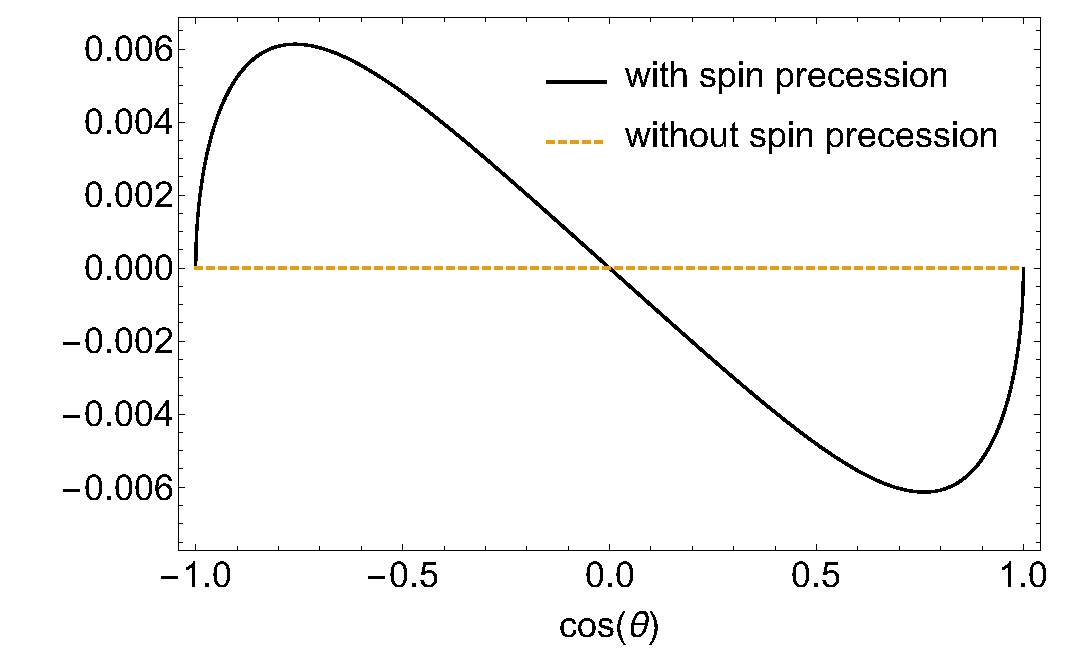
\includegraphics[width=0.9\linewidth]{figures/spin/px.eps}
    \caption{%
        $P_{\Lambda}^{y}$的分布。
    }%
    \label{fig:px}
\end{figure}
\section{蒙特卡洛模拟分析}
在实验上,自旋进动效应常常被忽略。在本节中,我们将利用蒙特卡洛模拟来研究忽略自旋进动效应带来的实验偏差。
参数$\alpha_{\psi}$, $\Phi$及$\alpha_{\pm}$的值的选择根据文献\cite{Ablikim:2018zay}的测量结果。
在模拟中不考虑任何$CP$破坏来源,假定$\alpha_{\pm}=\pm0.750$,同时
令$\alpha_{\psi}=0.462$, $\Phi=0.738$。探测器内部的磁场强度设为1T,对撞能点为$\sqrt{s} = $ 3.097 GeV, $\Lambda$
的动量为$\sqrt{s/4 - m^2}$。

蒙特卡洛产生子的基于ROOT\cite{ROOT}框架实现。在相空间事例的基础上,用形状\ref{eq:pdf}去随机舍取
一定的事例以得到蒙特卡洛样本。

为了揭示自旋进动效应对参数$\alpha_{\psi}$, $\Phi$ 和$\alpha_{\pm}$的影响,特别是对$CP$破坏测量的
影响, 对蒙特卡洛样本进行拟合以得到相应的参数值。几率密度函数的定义为
\begin{equation}
    \mathcal{P} = \frac{1}{N} \frac{{\rm d} \sigma}
    {{\rm d } \cos\theta {\rm d} \Omega_1 {\rm d} \Omega_2},
\end{equation}
式中$N$是归一化常数。经过积分得到其大小为$(4\pi){}^{2}(1 + \alpha_{\psi}/3)$。随后得到似然函数为:
\begin{equation}
    - \ln\mathcal{L} = -\sum_{i=1}^{n} \ln \mathcal{P}_{i},
\end{equation}
式中$i$代表蒙特卡洛样本中的第$i$个事例,$n$是样本的总事例数,其值为$1 \times 10^{6}$。
为了更好的区分,我们用脚标${}^{\rm truth}$表示基于修正后的形状\ref{eq:pdf}的拟合值,
而用脚标${}^{\rm biased}$表示基于未考虑自旋进动效应的形状的拟合值。
两组值之间的差异为:
\begin{equation}
    \begin{aligned}
        %\Delta \alpha &= \alpha^{\rm corr} - \alpha^{\rm exp}\\
        %\Delta \Phi  &= \Phi^{\rm corr} - \Phi^{\rm exp}\\
        \Delta \alpha_{\pm} & = \alpha_{\pm}^{\rm biased} - \alpha_{\pm}^{\rm truth} 
    \end{aligned}
\end{equation}

\begin{figure}[h!]
    \centering
    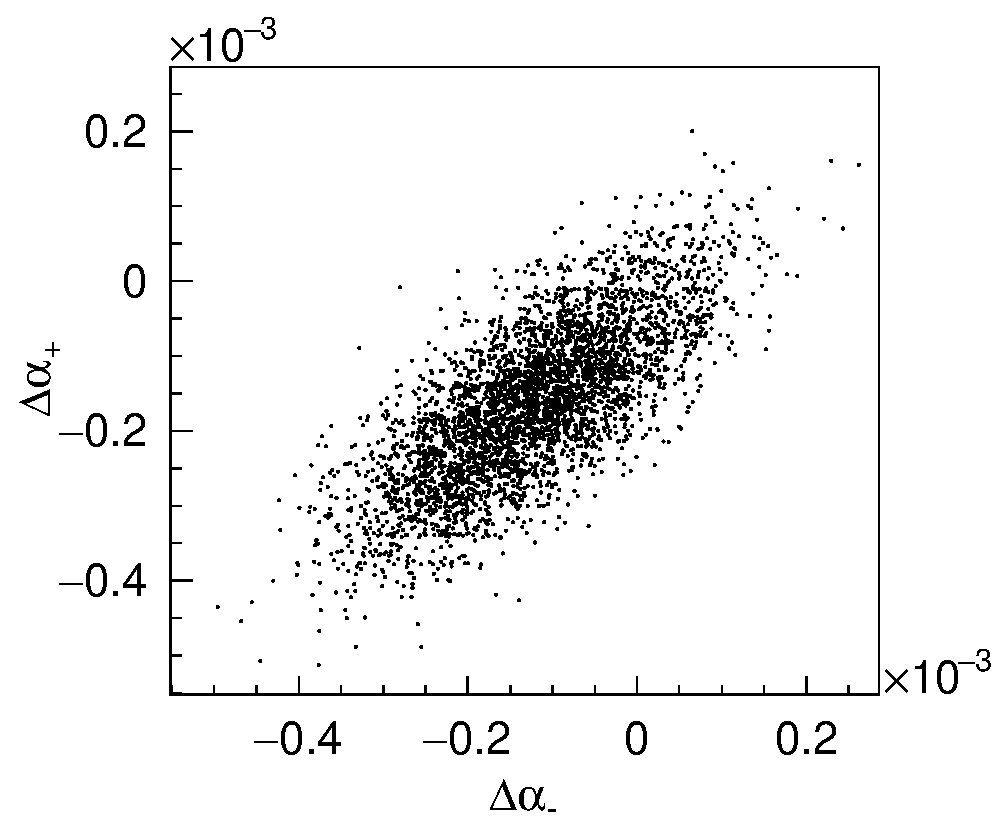
\includegraphics[width=0.8\linewidth]{figures/spin/corr.eps}
    \caption{%
        $\Delta \alpha_{-}$与$\Delta \alpha_{+}$之间的强关联。
 Each black point denotes the result from fitting to each toy MC sample.}%
    \label{fig:corr}
\end{figure}
我们产生了4000份蒙特卡洛样本,每个样本大小都相同,实验发现$\Delta \alpha_{-}$和$\Delta \alpha_{+}$之间有强烈的
关联,如图\ref{fig:corr}所示,图中的每个黑色的点均为一次实验的结果,点的疏密分布显示出很强的相关性。
这个强相关性将导致对$CP$破坏测量出现一定的偏差:
\begin{equation}
    \begin{split}
       \Delta A_{CP} &= \frac{1}{n}  \sum_{i=1}^{n} 
         \frac{\Delta \alpha_{-, i} + \Delta \alpha_{+, i}}
         {\alpha_{-, i}^{\rm biased} - \alpha_{+, i}^{\rm biased}} \\
        &=  (-1.9 \pm 0.1) \times 10^{-4}, 
    \end{split}
\end{equation}
式中$i$表示对第$i$个蒙特卡洛样本的结果, $n=4000$是实验的总次数。
这里使用了$CP$守恒条件,即$\alpha_{-}^{\rm truth} + \alpha_{+}^{\rm truth} =0$。
由此得到的$\Delta A_{CP}$大小是标准模型预言值的若干倍,正如图\ref{fig:acp}展示的。 
当增大磁场的强度时,如图\ref{fig:varyB}所示,和预期一致,$\Delta A_{CP}$的大小几乎线性地增加。
同时我们也观测到$\alpha_{\psi}$和$\Phi$也会分别偏离约0.07\% 和 0.01\%。
\begin{figure}[htpb]
    \centering
        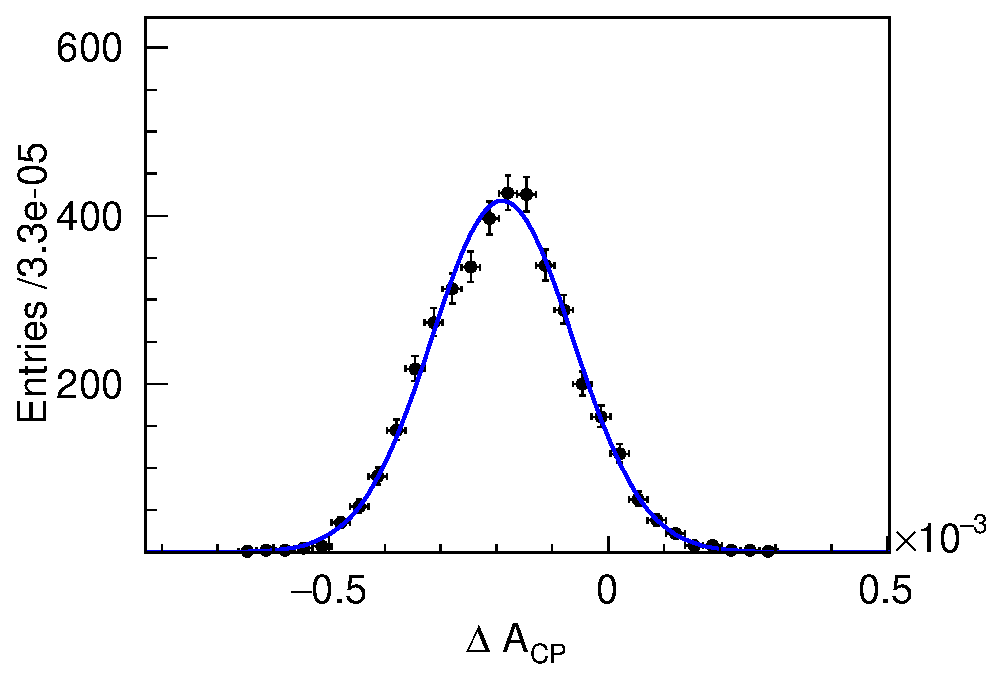
\includegraphics[width=0.9\linewidth]{figures/spin/afit.eps}
        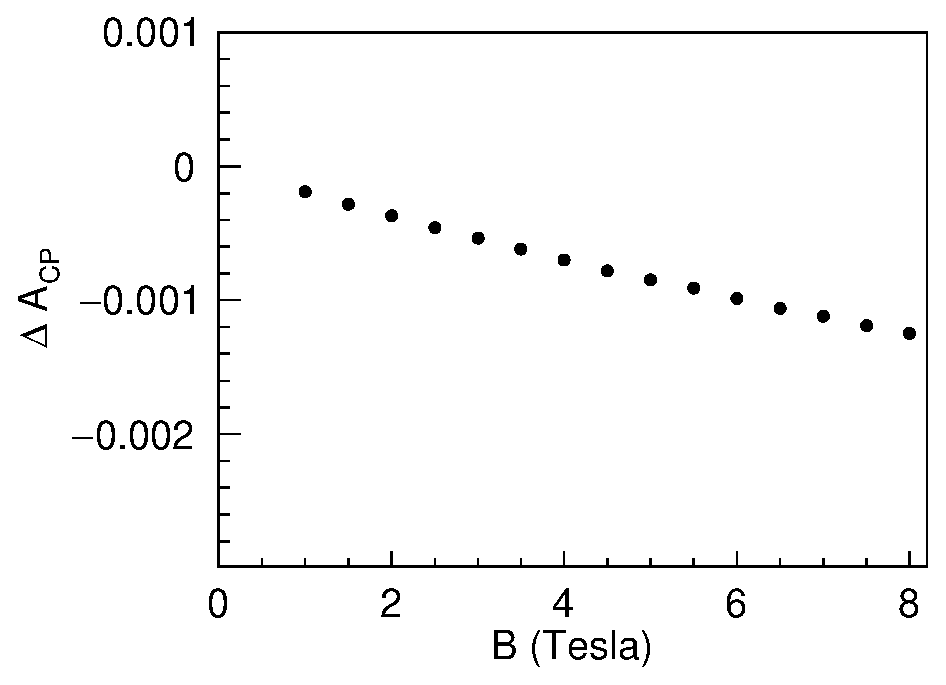
\includegraphics[width=0.9\linewidth]{figures/spin/Acp.eps}
    \caption{(a)$\Delta A_{CP}$的分布。 
    (b) 增大探测器内部的磁场的强度。}%
    \label{fig:acpandvaryB}
\end{figure}
\section{总结和讨论}
本章节考虑了磁场对超子对角分布的影响。由于超子存在磁矩,引起其自旋方向将会绕磁场转动,考虑
到这项修正,我们得到了整体的微分截面,微分截面的修正项与$\Lambda$的寿命成正比。
通过蒙特卡洛模拟,本节定量的考虑了磁场修正项的影响,并得到了一个重要的结论:一旦忽略磁场的影响,
实验上对 $CP$破坏的测量将不可避免的引入$10^{-4}$的偏差,这个偏差和标准模型预言的$CP$破坏大小相当。
于此同时,$\alpha_{\psi}$ 和 $\Phi$测量也会有微小的偏差,$\Lambda$的极化的观测也受到影响。

本文研究的这项效应,在其他的文献里\cite{Kharzeev:2015znc,Guo:2019joy,Deng:2018frf}也被研究了。
安装类似的方法,很容易把研究范围扩展到其他的超子对的产生,比如$\Xi\bar{\Xi}$, $\Sigma^{0}
\bar{\Sigma}^{0}$, $\Omega\bar{\Omega}$等。这个效应的影响比较小,目前的数据量有限不足以显示出
这项效应的影响, 但是在未来的超级粲陶工厂中,实验的灵敏度可达到$10^{-4}$甚至$10^{-5}$\cite{Bigi:2017eni},
这个效应的影响将起重要作用。 
